% ============================================================
% 4.2 PERSISTENCE AND PREDICTION -- Writer: Ignacio Gimeno -- about 460 words
% THIS IS THE CORE ML RESULT AND THE ANSWER TO IDRIS ("what the model is,
% errors, tuning"). Every model in Table~\ref{tab:models} must be discussed, including what
% the tuning curves (Figure~\ref{fig:tuning}, file fig8_model_tuning) say.
% Numbers: results/progress_stats.json (persistence), results/model_selection_stats.json,
% results/model_selection_tuning.csv, results/final_figures_stats.json (fig2, fig8),
% figures/final/CAPTIONS.md (entries fig2 and fig8). Outline entries 6b and 6c.
% ============================================================

\subsection{University Profiles Persist and Predict Unseen Years}
\label{sec:res-prediction}

\guide{Ignacio -- Paragraph: persistence (Figure~\ref{fig:persistence})}{%
\textbf{Claim (outline 6b):} the university-specific part is stable over time.\\
\textbf{Numbers:} correlation between a field's university-specific deviation in consecutive years $r = 0.84$ (95\% CI 0.84--0.85), 10,413 pairs; least-squares slope 0.85, close to the dashed line of perfect persistence.\\
\textbf{Interpretation:} a stable pattern is what makes prediction possible, and also what makes a correction based on past years usable (\S\ref{sec:res-adjusted}).}
\budget{100}{Ignacio}

\begin{figure}[t]
  \centering
  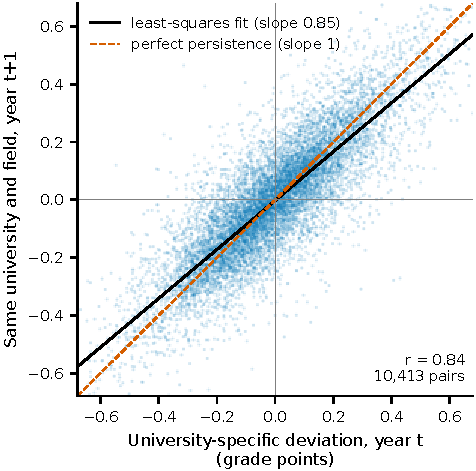
\includegraphics[width=0.92\linewidth]{fig2_persistence}
  \caption{\capguide{Ignacio -- see CAPTIONS.md, entry "Figure 2" (file fig2): what each point is (one university and field, two consecutive years), $r$ and number of pairs, meaning of the black and dashed red lines, units.}}
  \label{fig:persistence}
\end{figure}

\guide{Ignacio -- Paragraph: test errors (Table~\ref{tab:models})}{%
\textbf{Claim (outline 6c):} the university's own past is the best predictor of unseen years.\\
\textbf{Numbers (test 2022--2023):} baseline 0.365; common field effect 0.225; shrunk profile 0.138 (95\% CI 0.128--0.149); ridge 0.138; boosting 0.133. University profiles cut the error by 39\% relative to the shared effect; the paired bootstrap difference is $-0.098$ to $-0.077$ points, so the improvement is clear. $R^2$ rises from 0.62 to 0.86.\\
\textbf{Interpretation:} the 28\% university-specific share in \S\ref{sec:res-field} is real signal, not noise, because it predicts years the models never saw.}
\budget{130}{Ignacio}

% Table 2 -- prediction models. Numbers from results/model_selection_stats.json
% and results/model_selection_tuning.csv (checked 20 Nov 2026). Rounded to 3 d.p.
% Full grids: k in {0, 0.25, 0.5, 1, 2, 3, 5, 8, 13, 21, 50, inf}; alpha: 16
% log-spaced values from 1e-2 to 1e3; boosting: depth {2,3,5,8} x learning rate
% {0.03, 0.1, 0.3} x trees {100, 300, 600}.
\begin{table*}[t]
\centering
\caption{Prediction of a field's deviation from its university-year average, $d_{ufy}$, in grade points. Models are trained on 2015--2021, tuned by expanding-window validation on 2018--2021 (Algorithm~\ref{alg:tuning}; grids in \S\ref{sec:methods-prediction}) and evaluated once on 2022--2023 (2,774 university-field-years, 87 universities). The 95\% intervals come from 1,000 bootstrap resamples of universities. Lower RMSE and MAE are better.}
\label{tab:models}
\footnotesize
\setlength{\tabcolsep}{3.5pt}
\begin{tabular}{@{}lllcccc@{}}
\toprule
Model & Grid searched & Chosen & Valid.\ RMSE & Test RMSE (95\% CI) & Test MAE & Test $R^2$ \\
 & & & 2018--2021 & 2022--2023 & & \\
\midrule
Baseline (predict 0) & -- & -- & 0.360 & 0.365 (0.348--0.381) & 0.296 & 0.00 \\
Common field effect & -- & -- & 0.219 & 0.225 (0.211--0.241) & 0.174 & 0.62 \\
Shrunk university profile & 12 values, 0 to $\infty$ & $k = 0.25$ & 0.116 & 0.138 (0.128--0.149) & 0.103 & 0.86 \\
Ridge (field, university$\times$field) & 16 values, $10^{-2}$ to $10^{3}$ & $\alpha = 0.22$ & 0.116 & 0.138 (0.129--0.149) & 0.103 & 0.86 \\
Gradient boosting & 36 (depth, rate, trees) & 8, 0.03, 600 & 0.114 & 0.133 (0.123--0.143) & 0.098 & 0.87 \\
\bottomrule
\end{tabular}
\end{table*}


\guide{Ignacio -- Paragraph: what tuning shows (Figure~\ref{fig:tuning})}{%
\textbf{(a) Shrinkage:} the best $k$ is small (0.25): with up to seven past years, the university's own history deserves almost full weight; as $k$ grows the error rises towards the shared-effect line, which is the case $k=\infty$.\\
\textbf{(b) Ridge:} chosen $\alpha = 0.22$; same error as the shrunk profile (0.138) because both are forms of partial pooling -- a useful check that the result does not depend on one implementation. Large $\alpha$ removes the university terms and the error climbs.\\
\textbf{(c) Boosting:} the curve is almost flat (validation 0.116 at depth 2, 0.114 at depth 8); the chosen model (depth 8, rate 0.03, 600 trees) is at the edge of the grid, but the flat curve shows that larger models would gain little.}
\budget{130}{Ignacio}

\begin{figure*}[t]
  \centering
  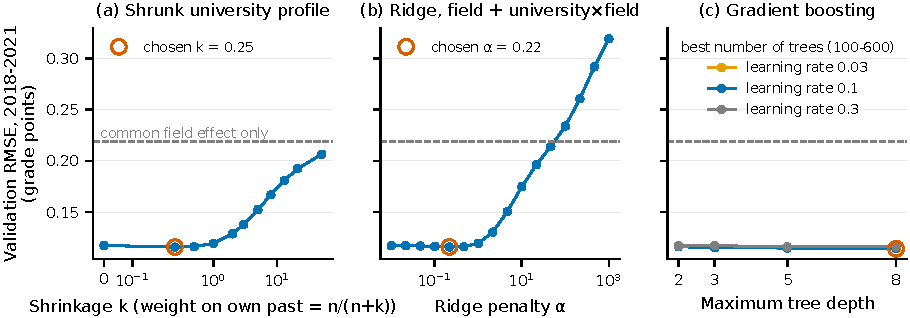
\includegraphics[width=\textwidth]{fig8_model_tuning}
  \caption{\capguide{Ignacio -- see CAPTIONS.md, entry "Figure 8" (file fig8): expanding-window validation error (2018--2021, grade points) for each value of the tuned hyperparameter; the red circle is the chosen value; dashed grey line = common field effect only; test years never used.}}
  \label{fig:tuning}
\end{figure*}

\guide{Ignacio -- Paragraph: which model we keep and why}{%
\textbf{Decision:} boosting is better than the shrunk profile by only 0.002--0.008 points (paired bootstrap, about 3\%), while the shrunk profile has one parameter and a direct reading (weight $n/(n+k)$ on the university's own past). We keep the shrunk profile for interpretation and for the adjusted mark. Boosting can also use dropout and size, yet it improves only slightly; do not claim more than that (no separate test removed those two features).\\
\textbf{Link:} the same idea -- use a university's past deviation -- is what makes the adjusted mark in \S\ref{sec:res-adjusted} work.}
\budget{100}{Ignacio}
